% Selected simulation evidence regenerated by the unified branch.

\subsubsection{Current terminal distribution and latent-state diagnostics}

The current Team~8 diagnostic simulation uses the 2 September calibration
with $q=0.40\%$, regenerated on 24 October 2026 with the corrected path
engines: 4,096 paths, 260 weekly steps over five years and the GLD level
402.78 USD/share. Its constant annual rate is 4.0770\%, so the drift is
$r-q=3.6770\%$. This standalone state-law illustration differs from the
corporate adapter, which starts from the XAUUSD spot of USD~4,391.32/oz at the
valuation time and uses daily steps, integral-preserving NSS forward rates and
8,192 paths. Neither the levels nor the path percentiles are interchangeable.

\begin{table}[H]
\centering
\scriptsize
\setlength{\tabcolsep}{2.45pt}
\begin{tabular}{@{}lrrrrrrrr@{}}
\toprule
Model & Mean & Std & P05 & P50 & P95 & Return skew & Ex. kurt. & Mean jumps \\
\midrule
GBM / BS & 481.438 & 302.612 & 155.071 & 406.941 & 1065.891 & 1.963 & 6.821 & 0.000 \\
Heston & 483.698 & 316.776 & 143.485 & 415.373 & 1047.567 & 2.419 & 11.587 & 0.000 \\
Bates & 483.676 & 301.643 & 138.647 & 414.135 & 1042.365 & 1.912 & 6.684 & 8.619 \\
Full Bates--Hawkes & 487.072 & 442.287 & 140.206 & 404.316 & 1043.533 & 15.209 & 470.483 & 8.346 \\
\bottomrule
\end{tabular}
\caption{Terminal GLD price and simple-return diagnostics regenerated from the
current Team 8 calibration ($q=0.40\%$): 4,096 five-year paths, 260 weekly
steps and a fixed seed (Article~8 \texttt{terminal\_path\_stats.csv}). The
jump models mainly alter tail shape and event counts. Full Bates--Hawkes has
a much fatter right tail: excess return kurtosis 470 and a maximum simple
return of about 4,007\%, driven by a few clustered jump paths, while its
P05--P95 range is close to the other models. These levels are not Barrick
values and are not inputs to the later 8,192-path corporate comparison.}
\label{tab:t8-terminal-path-stats}
\end{table}

\begin{figure}[p]
    \centering
    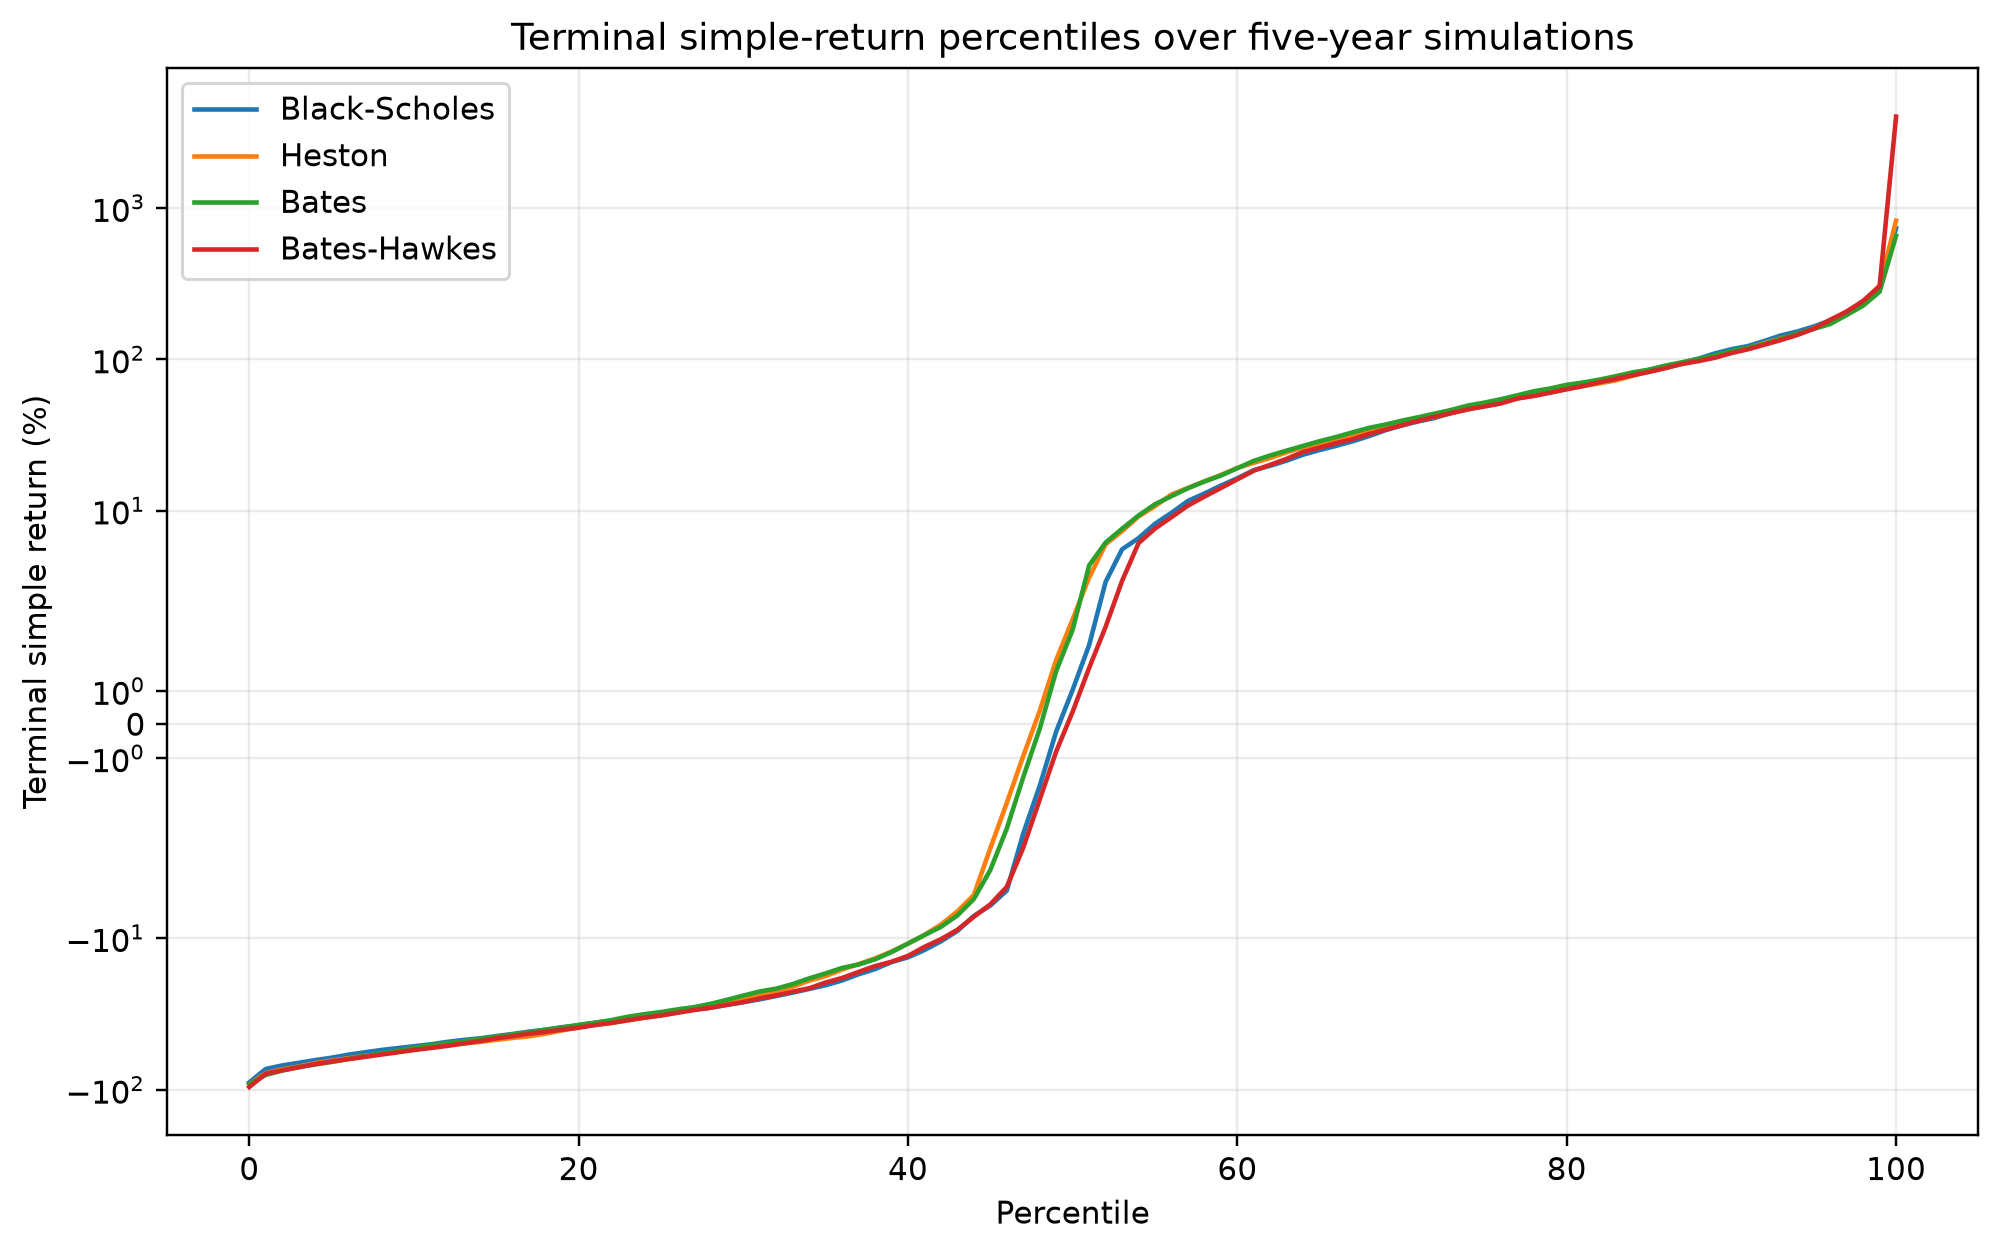
\includegraphics[width=0.94\textwidth]{../img/publication/14370a1fa55e1d67_terminal_return_percentiles.png}
    \caption{All integer percentiles 0--100 of five-year simple GLD returns in
    the current Team 8 simulation ($q=0.40\%$, corrected engines). The symmetric-log scale retains the
    central distribution while exposing extreme endpoints; the full integer
    percentile tables remain in the source article rather than being repeated
    in the thesis.}
    \label{fig:t8-terminal-return-percentiles}
\end{figure}

\begin{figure}[p]
    \centering
    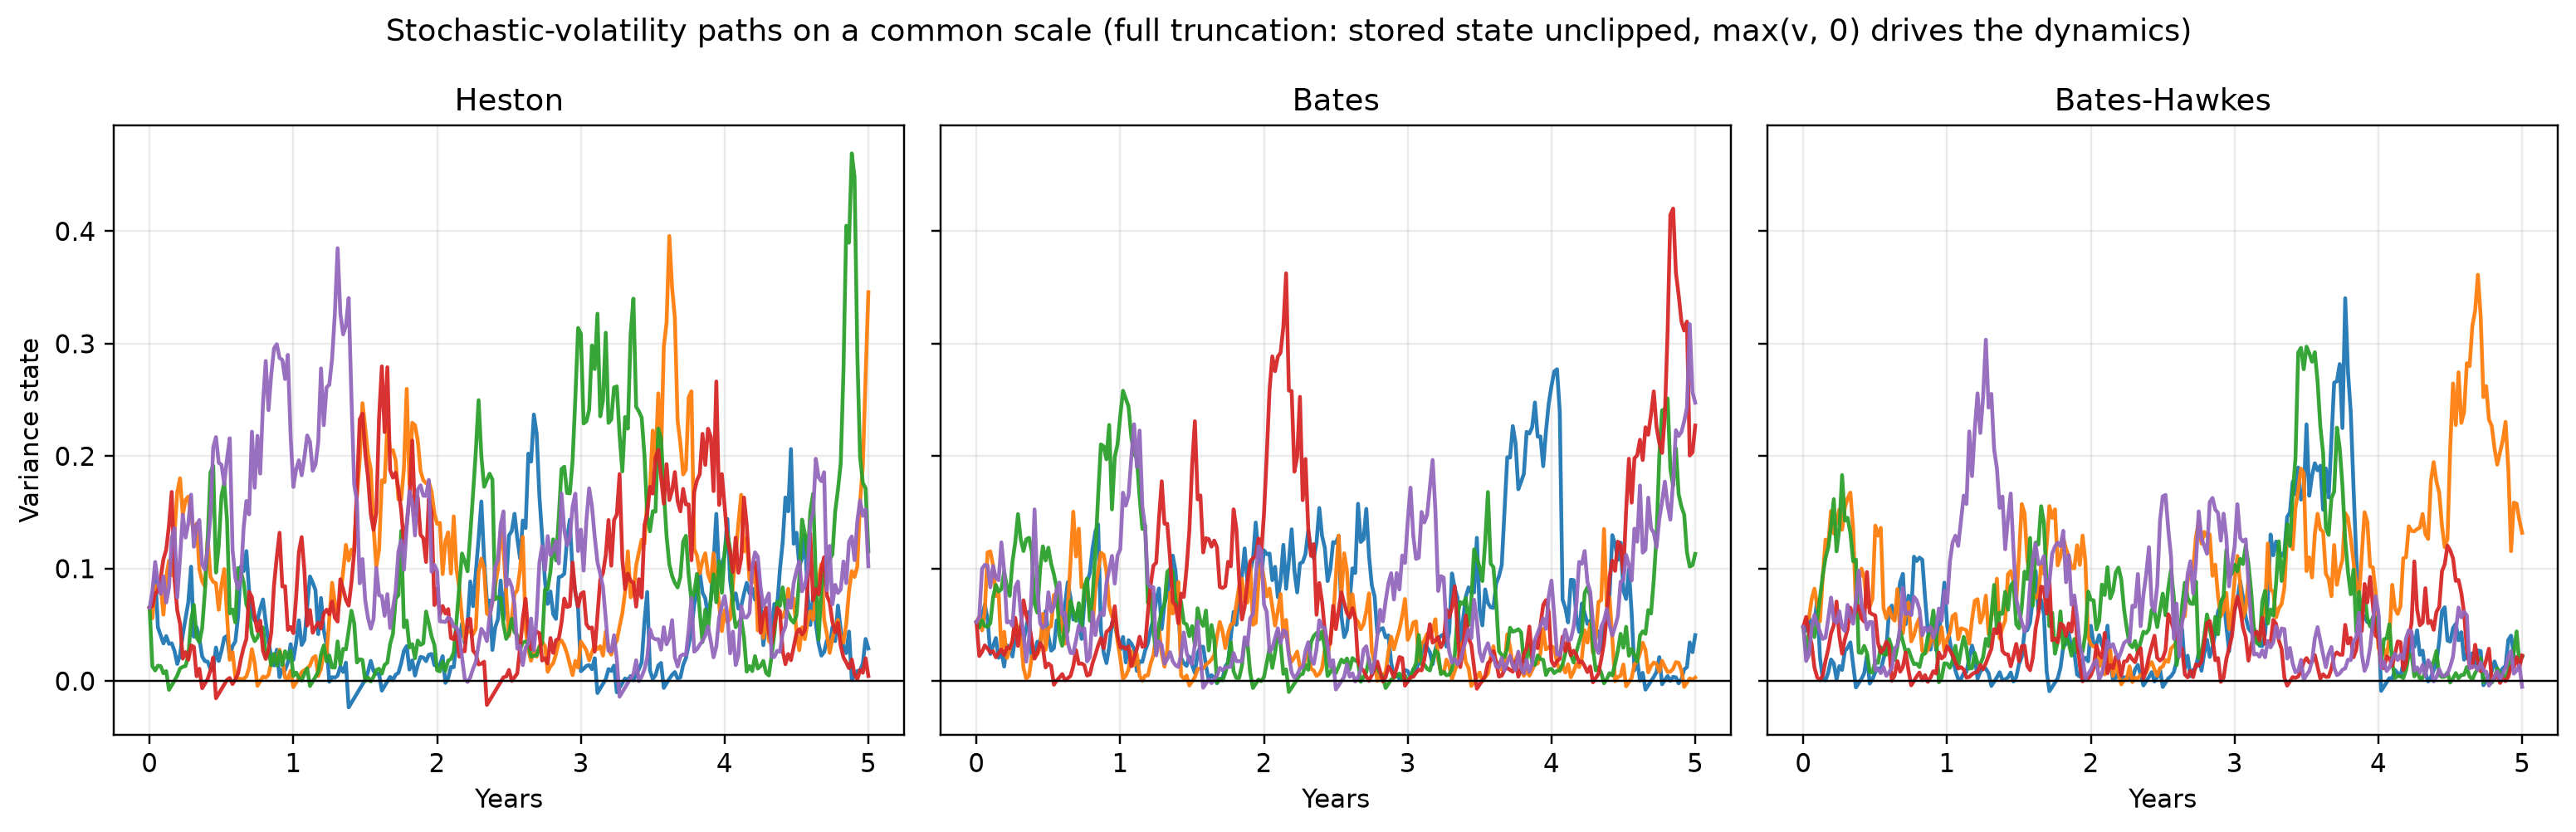
\includegraphics[width=0.98\textwidth]{../img/publication/fbaa0a114c49c80a_volatility_state_paths.png}
    \caption{Representative variance-state paths under Heston, Bates and Full
    Bates--Hawkes on a common scale ($q=0.40\%$ calibration). Under full
    truncation the stored state is unclipped and can dip slightly below zero;
    only $\max(v,0)$ drives the dynamics. The plot verifies that all three
    richer engines carry a simulated variance state; the jump mechanism does
    not replace stochastic variance.}
    \label{fig:t8-volatility-state-paths}
\end{figure}

\begin{figure}[p]
    \centering
    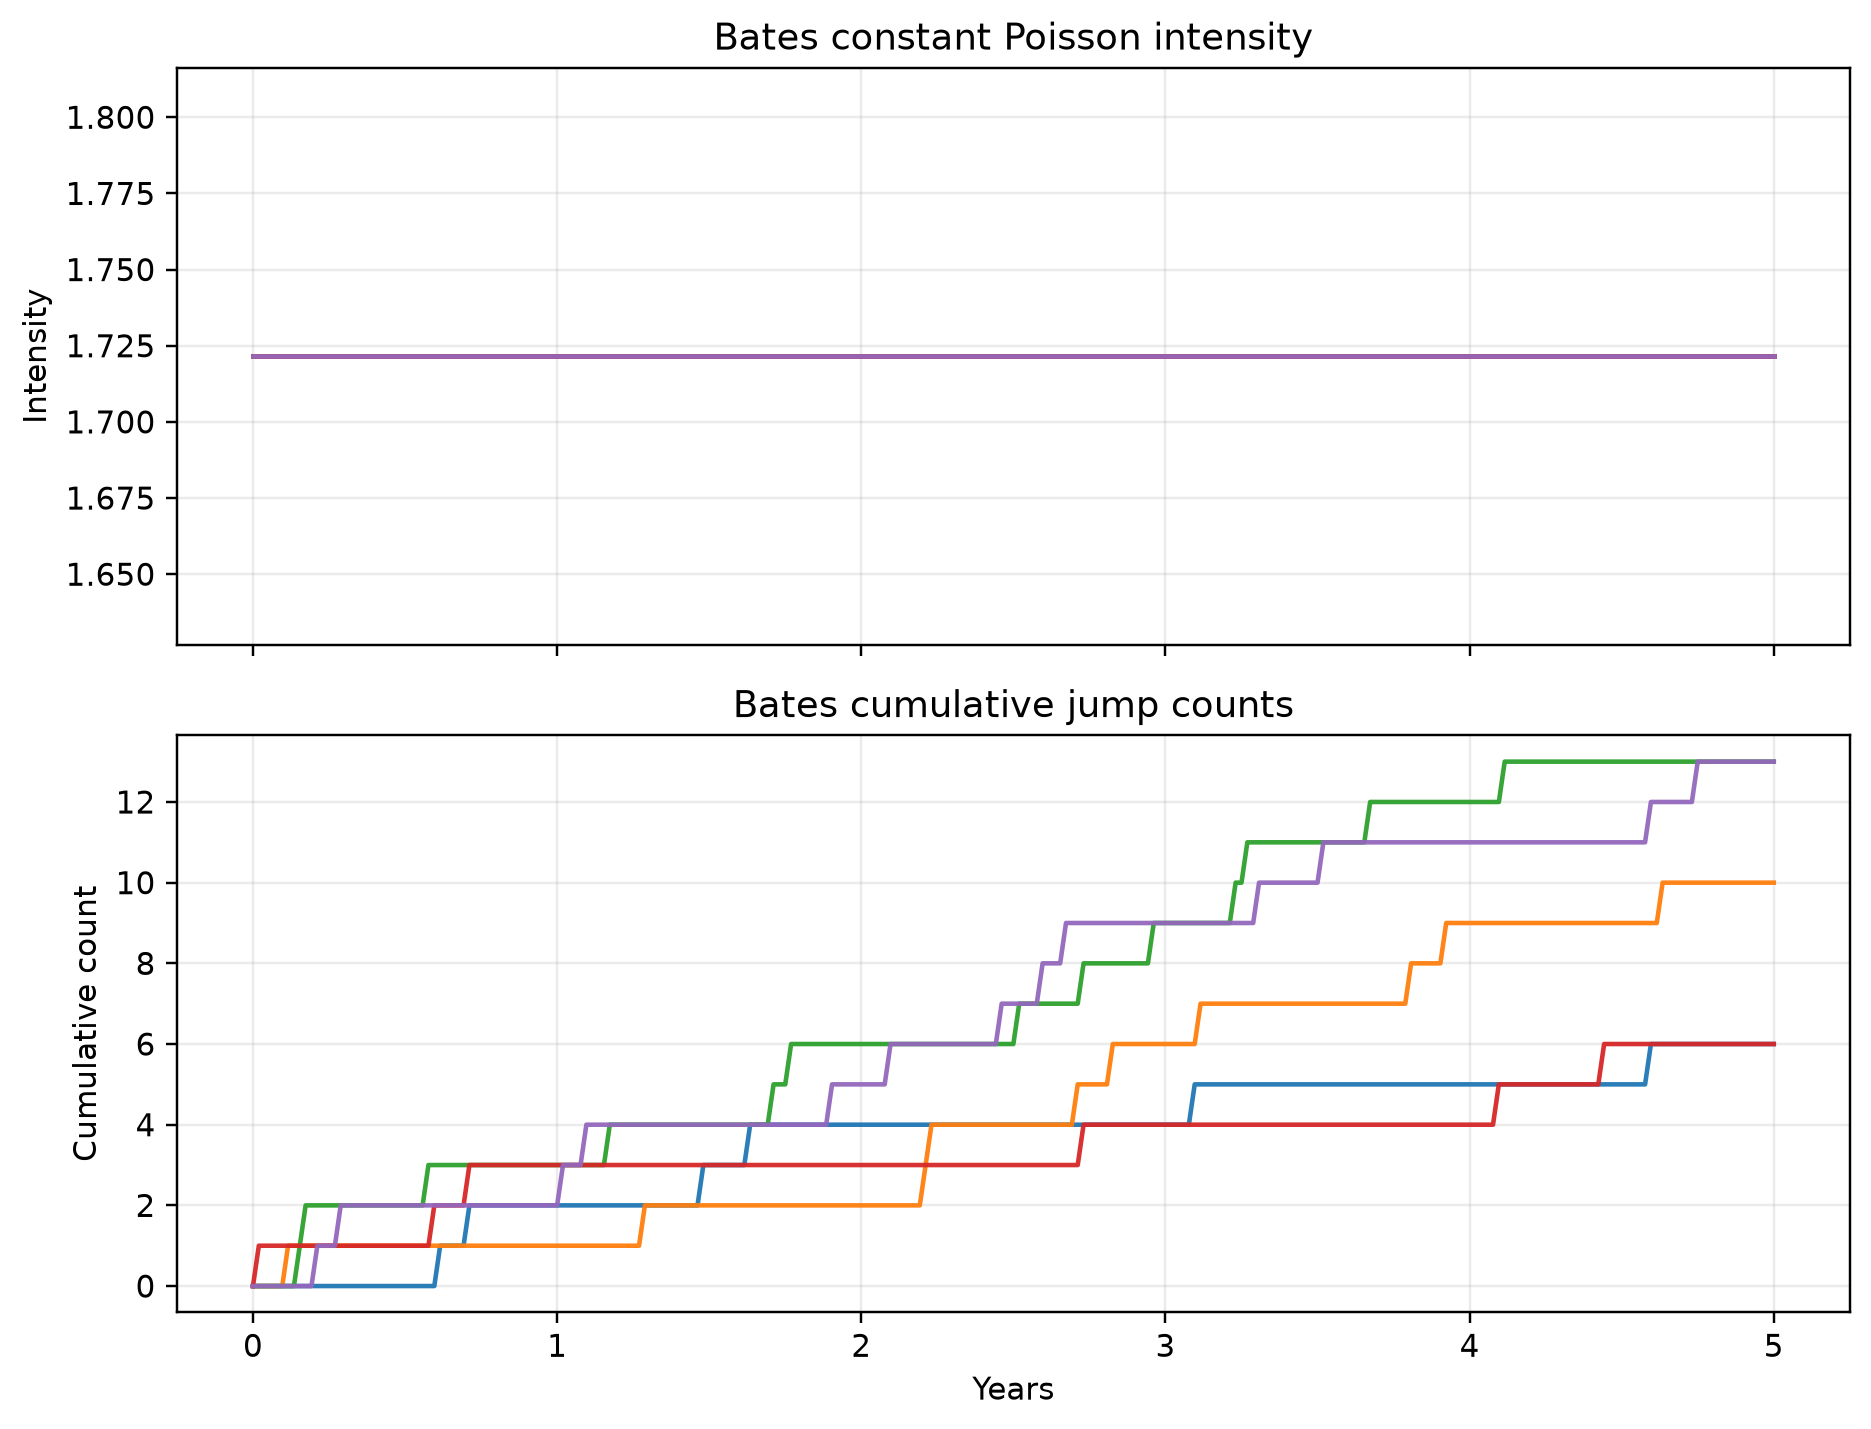
\includegraphics[width=0.68\textwidth]{../img/publication/3365b35f410bfed1_bates_poisson_jump_paths.png}

    \vspace{3mm}
    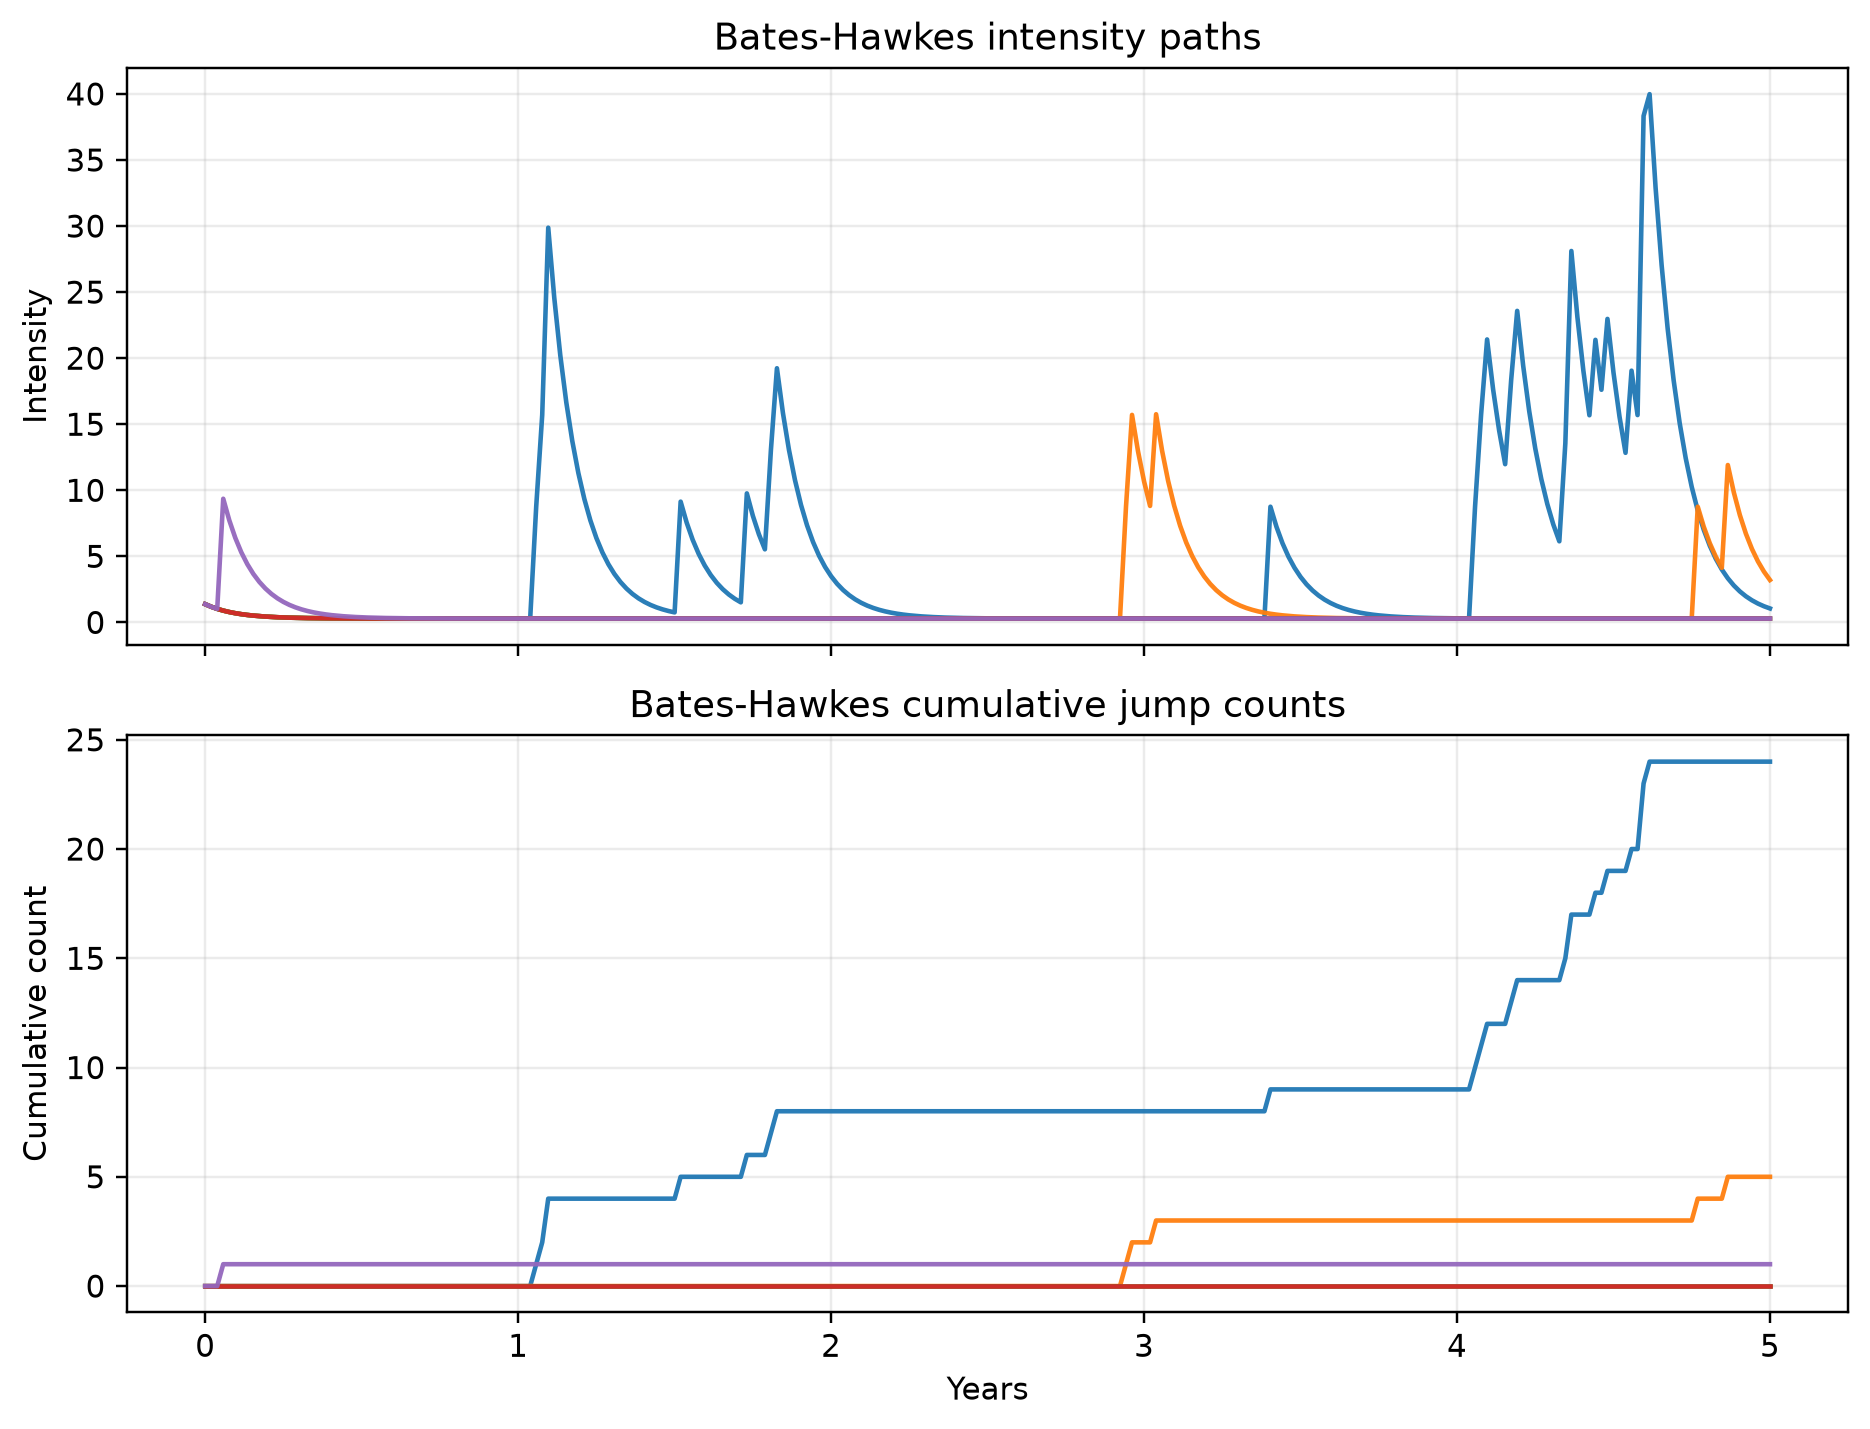
\includegraphics[width=0.68\textwidth]{../img/publication/e5bf0d6a1e149452_hawkes_jump_paths.png}
    \caption{Representative jump-state diagnostics regenerated from the
    $q=0.40\%$ calibration with the exact Hawkes intensity integral. Top: Bates retains a
    constant Poisson intensity while cumulative counts evolve independently.
    Bottom: Full Bates--Hawkes intensity rises after arrivals and decays toward
    its baseline, generating clustered event counts. These path displays
    explain the state difference behind the tail comparison; they are not
    additional forecast observations.}
    \label{fig:t8-jump-state-comparison}
\end{figure}
